\documentclass[11pt, letterpaper]{article}

% Fonts and Encoding
\usepackage[utf8]{inputenc}
\usepackage[T1]{fontenc}
\usepackage{lmodern} % High-quality Latin Modern vector font

% Math and Symbols
\usepackage{amsmath, amssymb, amsthm, amsfonts, mathrsfs, mathtools}

% Layout and Geometry
\usepackage{geometry}
\geometry{letterpaper, margin=1in}
\setlength{\parindent}{0pt}
\setlength{\parskip}{0.6em}

% Formatting and Graphics
\usepackage{graphicx, xcolor, enumitem, booktabs, array, tabularx}

% TikZ for Illustrations
\usepackage{tikz}
\usetikzlibrary{arrows.meta, positioning, shapes.geometric, calc, backgrounds, matrix}

% Clickable Links and TOC
\usepackage{hyperref}
\hypersetup{
    colorlinks=true,
    linkcolor=blue,
    filecolor=magenta,      
    urlcolor=cyan,
    pdftitle={Advanced Mathematics Topic},
}

% Theorem Environments
\newtheorem{theorem}{Theorem}[section]
\newtheorem{lemma}[theorem]{Lemma}
\newtheorem{proposition}[theorem]{Proposition}
\newtheorem{corollary}[theorem]{Corollary}
\theoremstyle{definition}
\newtheorem{definition}{Definition}[section]
\newtheorem{axiom}{Axiom}[section]
\newtheorem{example}{Example}[section]
\theoremstyle{remark}
\newtheorem{remark}{Remark}[section]

% Custom Commands (Enforced standard notation)
\newcommand{\R}{\mathbb{R}}
\newcommand{\N}{\mathbb{N}}
\newcommand{\Z}{\mathbb{Z}}
\newcommand{\Q}{\mathbb{Q}}
\newcommand{\E}{\mathbb{E}}
\newcommand{\Prob}{\mathbb{P}}
\newcommand{\F}{\mathcal{F}}

\title{\textbf{Machine Learning and Linear Models \\ \Large A Comprehensive Study Guide and Solution Manual}}
\author{Tashfeen Omran}
\date{\today}

\begin{document}

\maketitle
\tableofcontents
\newpage

\section{Part 1: Comprehensive Introduction, Context, and Prerequisites}

\subsection{Core Concepts}
The topic of \textbf{Machine Learning and Linear Models} (often framed within the context of Inner Product Spaces and Orthogonality) bridges the gap between abstract linear algebra and applied data science. At its core, it addresses the problem of finding the "best fit" for a set of data points that do not perfectly align due to noise, measurement error, or inherent variance. 

We introduce several key variables and notations:
\begin{itemize}
    \item $X$: The \textbf{design matrix}, containing the independent variables (inputs).
    \item $y$: The \textbf{observation vector}, containing the dependent variables (outputs).
    \item $\beta$: The \textbf{parameter vector}, containing the unknown coefficients we wish to learn.
    \item $\epsilon$: The \textbf{residual vector}, representing the error between the observed data and the model's predictions ($\epsilon = y - X\beta$).
\end{itemize}
The goal of linear regression is to find an optimal parameter vector $\hat{\beta}$ that minimizes the length (or squared norm) of the residual vector, $\|\epsilon\|^2 = \|y - X\beta\|^2$.

\subsection{Intuition and Derivation}
Geometrically, the matrix-vector product $X\beta$ represents a linear combination of the columns of $X$. Therefore, $X\beta$ must lie in the column space of $X$, denoted as $\text{Col } X$. If the observation vector $y$ does not lie perfectly in $\text{Col } X$ (which is almost always the case with real-world data), the system $X\beta = y$ has no exact solution.

To find the "closest" solution, we project $y$ orthogonally onto $\text{Col } X$. Let $\hat{y} = X\hat{\beta}$ be this projection. By the Orthogonal Decomposition Theorem, the residual vector $\epsilon = y - \hat{y}$ must be orthogonal to every vector in $\text{Col } X$. 
This means $\epsilon$ is in the null space of $X^T$, yielding the fundamental relationship:
\[ X^T (y - X\hat{\beta}) = 0 \implies X^T X \hat{\beta} = X^T y \]
These are the \textbf{Normal Equations}. Solving them gives the least-squares parameters $\hat{\beta}$.

\begin{center}
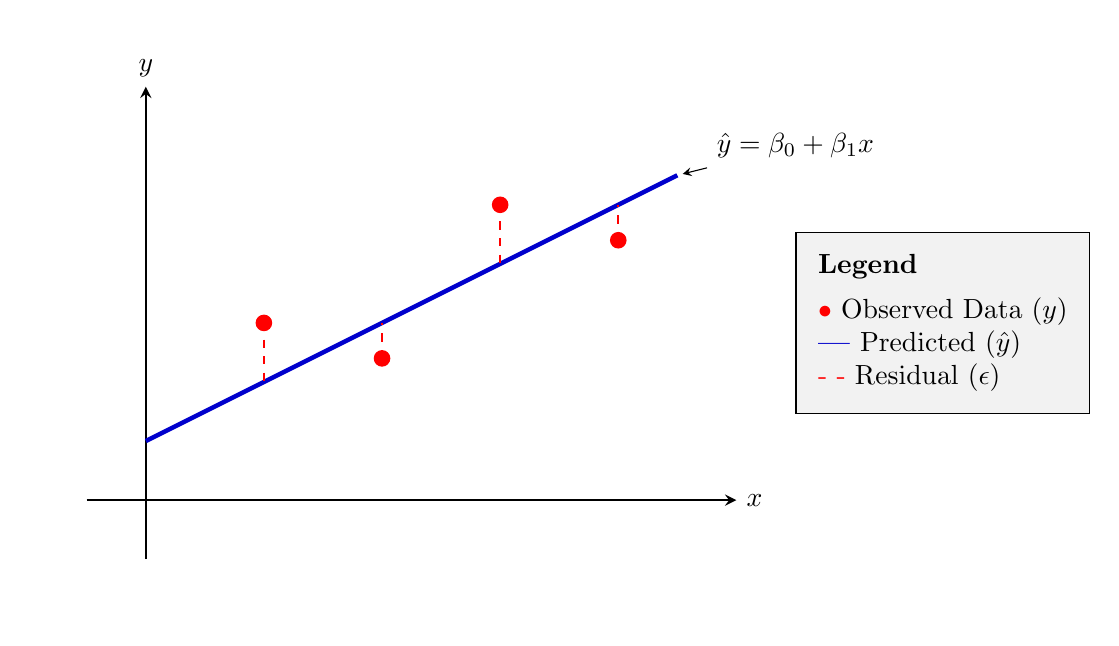
\begin{tikzpicture}[scale=1.5]
    % Background to ensure layering
    \fill[white] (-1,-1) rectangle (7,4);
    
    % Axes
    \draw[thick, ->, >=stealth] (-0.5, 0) -- (5, 0) node[right, black] {$x$};
    \draw[thick, ->, >=stealth] (0, -0.5) -- (0, 3.5) node[above, black] {$y$};
    
    % Regression Line
    \draw[ultra thick, blue!80!black] (0, 0.5) -- (4.5, 2.75) coordinate (line_end);
    
    % Callout for the line
    \node[black] at (5.5, 3) (eq) {$\displaystyle \hat{y} = \beta_0 + \beta_1 x$};
    \draw[->, >=stealth, shorten >=2pt] (eq) -- (line_end);
    
    % Data points and residuals
    \coordinate (P1) at (1, 1.5);
    \coordinate (L1) at (1, 1.0);
    \fill[red] (P1) circle (2pt);
    \draw[dashed, thick, red] (P1) -- (L1);
    
    \coordinate (P2) at (2, 1.2);
    \coordinate (L2) at (2, 1.5);
    \fill[red] (P2) circle (2pt);
    \draw[dashed, thick, red] (P2) -- (L2);
    
    \coordinate (P3) at (3, 2.5);
    \coordinate (L3) at (3, 2.0);
    \fill[red] (P3) circle (2pt);
    \draw[dashed, thick, red] (P3) -- (L3);
    
    \coordinate (P4) at (4, 2.2);
    \coordinate (L4) at (4, 2.5);
    \fill[red] (P4) circle (2pt);
    \draw[dashed, thick, red] (P4) -- (L4);
    
    % Legend
    \node[align=left, anchor=west, inner sep=8pt, draw, fill=gray!10] at (5.5, 1.5) {
        \textbf{Legend} \\[4pt]
        \textcolor{red}{$\bullet$} Observed Data ($y$) \\
        \textcolor{blue!80!black}{\textbf{---}} Predicted ($\hat{y}$) \\
        \textcolor{red}{- -} Residual ($\epsilon$)
    };
\end{tikzpicture}
\end{center}

\subsection{Historical Context and Motivation}
The method of least squares was independently developed by Carl Friedrich Gauss and Adrien-Marie Legendre in the early 19th century. Its most famous early application occurred in 1801 when Gauss used it to predict the orbit of the newly discovered asteroid Ceres. After Ceres passed behind the sun and was lost to astronomers, Gauss applied his least-squares technique to the limited available data, successfully predicting its exact location when it re-emerged months later. This established least squares as a foundational tool in astronomy, geodesy, and eventually, modern machine learning.

\subsection{Key Formulas}
\begin{itemize}
    \item \textbf{The Linear Model:} $y = X\beta + \epsilon$
    \item \textbf{The Normal Equations:} $X^T X \hat{\beta} = X^T y$
    \item \textbf{Least-Squares Solution (if $X^T X$ is invertible):} $\hat{\beta} = (X^T X)^{-1} X^T y$
    \item \textbf{Predicted Values:} $\hat{y} = X\hat{\beta}$
    \item \textbf{Sum of Squared Errors (SSE):} $\|\epsilon\|^2 = \|y - \hat{y}\|^2 = (y - X\hat{\beta})^T (y - X\hat{\beta})$
\end{itemize}

\subsection{Prerequisites}
To master this topic, you must be proficient in:
1. \textbf{Matrix Algebra:} Matrix multiplication, transposes, and inverses.
2. \textbf{Orthogonality:} Understanding dot products, orthogonal complements, and projections in $\R^n$.
3. \textbf{Calculus (Optional but helpful):} Understanding that minimizing the squared error function via partial derivatives yields the exact same Normal Equations derived via linear algebra.

\newpage
\section{Part 2: Detailed Homework Solutions}

\textit{Note: To maximize learning efficiency, a strategic selection of 10 problems has been chosen from the text. This selection covers at least two of every distinct problem archetype (Simple Linear, Polynomial/Multiple, Transformations, Predictions, and Theoretical Proofs), ensuring complete conceptual coverage without redundant repetition.}

% --- PROBLEM 1 ---
\subsection*{Problem 1 (Simple Linear Regression)}
\textbf{Problem Statement:} Find the equation $y = \beta_0 + \beta_1 x$ of the least-squares line that best fits the given data points: $(0, 1), (1, 1), (2, 2), (3, 2)$.

\textbf{Solution:}
First, we construct the design matrix $X$ and the observation vector $y$. Because the model is $y = \beta_0 + \beta_1 x$, the first column of $X$ consists of 1s (corresponding to the constant $\beta_0$), and the second column consists of the $x$-coordinates.
\[
X = \begin{bmatrix} 1 & 0 \\ 1 & 1 \\ 1 & 2 \\ 1 & 3 \end{bmatrix}, \quad y = \begin{bmatrix} 1 \\ 1 \\ 2 \\ 2 \end{bmatrix}
\]
Next, we compute $X^T X$ and $X^T y$ to set up the normal equations $X^T X \hat{\beta} = X^T y$.
\begin{align*}
X^T X &= \begin{bmatrix} 1 & 1 & 1 & 1 \\ 0 & 1 & 2 & 3 \end{bmatrix} \begin{bmatrix} 1 & 0 \\ 1 & 1 \\ 1 & 2 \\ 1 & 3 \end{bmatrix} = \begin{bmatrix} 4 & 6 \\ 6 & 14 \end{bmatrix} \\ \relax
X^T y &= \begin{bmatrix} 1 & 1 & 1 & 1 \\ 0 & 1 & 2 & 3 \end{bmatrix} \begin{bmatrix} 1 \\ 1 \\ 2 \\ 2 \end{bmatrix} = \begin{bmatrix} 1+1+2+2 \\ 0+1+4+6 \end{bmatrix} = \begin{bmatrix} 6 \\ 11 \end{bmatrix}
\end{align*}
Now, we solve the system $\begin{bmatrix} 4 & 6 \\ 6 & 14 \end{bmatrix} \begin{bmatrix} \beta_0 \\ \beta_1 \end{bmatrix} = \begin{bmatrix} 6 \\ 11 \end{bmatrix}$. We find the inverse of $X^T X$:
\[
\det(X^T X) = (4)(14) - (6)(6) = 56 - 36 = 20
\]
\[
(X^T X)^{-1} = \frac{1}{20} \begin{bmatrix} 14 & -6 \\ -6 & 4 \end{bmatrix}
\]
Multiply by $X^T y$ to find $\hat{\beta}$:
\begin{align*}
\hat{\beta} &= \frac{1}{20} \begin{bmatrix} 14 & -6 \\ -6 & 4 \end{bmatrix} \begin{bmatrix} 6 \\ 11 \end{bmatrix} \\ \relax
&= \frac{1}{20} \begin{bmatrix} 14(6) - 6(11) \\ -6(6) + 4(11) \end{bmatrix} \\ \relax
&= \frac{1}{20} \begin{bmatrix} 84 - 66 \\ -36 + 44 \end{bmatrix} = \frac{1}{20} \begin{bmatrix} 18 \\ 8 \end{bmatrix} = \begin{bmatrix} 0.9 \\ 0.4 \end{bmatrix}
\end{align*}
\textbf{Final Answer:} The least-squares line is $\displaystyle y = 0.9 + 0.4x$.

% --- PROBLEM 2 ---
\subsection*{Problem 2 (Simple Linear Regression)}
\textbf{Problem Statement:} Find the equation $y = \beta_0 + \beta_1 x$ of the least-squares line that best fits the given data points: $(1, 0), (2, 2), (3, 7), (4, 9)$.

\textbf{Solution:}
Construct the design matrix $X$ and observation vector $y$:
\[
X = \begin{bmatrix} 1 & 1 \\ 1 & 2 \\ 1 & 3 \\ 1 & 4 \end{bmatrix}, \quad y = \begin{bmatrix} 0 \\ 2 \\ 7 \\ 9 \end{bmatrix}
\]
Compute $X^T X$ and $X^T y$:
\begin{align*}
X^T X &= \begin{bmatrix} 1 & 1 & 1 & 1 \\ 1 & 2 & 3 & 4 \end{bmatrix} \begin{bmatrix} 1 & 1 \\ 1 & 2 \\ 1 & 3 \\ 1 & 4 \end{bmatrix} = \begin{bmatrix} 4 & 10 \\ 10 & 30 \end{bmatrix} \\ \relax
X^T y &= \begin{bmatrix} 1 & 1 & 1 & 1 \\ 1 & 2 & 3 & 4 \end{bmatrix} \begin{bmatrix} 0 \\ 2 \\ 7 \\ 9 \end{bmatrix} = \begin{bmatrix} 0+2+7+9 \\ 0+4+21+36 \end{bmatrix} = \begin{bmatrix} 18 \\ 61 \end{bmatrix}
\end{align*}
Find the inverse of $X^T X$:
\[
\det(X^T X) = (4)(30) - (10)(10) = 120 - 100 = 20
\]
\[
(X^T X)^{-1} = \frac{1}{20} \begin{bmatrix} 30 & -10 \\ -10 & 4 \end{bmatrix}
\]
Calculate $\hat{\beta}$:
\begin{align*}
\hat{\beta} &= \frac{1}{20} \begin{bmatrix} 30 & -10 \\ -10 & 4 \end{bmatrix} \begin{bmatrix} 18 \\ 61 \end{bmatrix} \\ \relax
&= \frac{1}{20} \begin{bmatrix} 30(18) - 10(61) \\ -10(18) + 4(61) \end{bmatrix} \\ \relax
&= \frac{1}{20} \begin{bmatrix} 540 - 610 \\ -180 + 244 \end{bmatrix} = \frac{1}{20} \begin{bmatrix} -70 \\ 64 \end{bmatrix} = \begin{bmatrix} -3.5 \\ 3.2 \end{bmatrix}
\end{align*}
\textbf{Final Answer:} The least-squares line is $\displaystyle y = -3.5 + 3.2x$.

% --- PROBLEM 5 ---
\subsection*{Problem 5 (Model Prediction)}
\textbf{Problem Statement:} If a machine learns the least-squares line that best fits the data in Exercise 1, what will the machine pick for the value of $y$ when $x = 4$?

\textbf{Solution:}
From Problem 1, the learned least-squares line is $y = 0.9 + 0.4x$. 
To predict the value of $y$ for a new input $x = 4$, we simply substitute $x = 4$ into our linear model:
\begin{align*}
y &= 0.9 + 0.4(4) \\ \relax
y &= 0.9 + 1.6 \\ \relax
y &= 2.5
\end{align*}
\textbf{Final Answer:} The machine will predict $\displaystyle y = 2.5$.

% --- PROBLEM 9 ---
\subsection*{Problem 9 (Model Evaluation \& Extrapolation)}
\textbf{Problem Statement:} If you enter the data from Exercise 1 into a machine and it returns a $y$ value of 20 when $x = 2.5$, should you trust the machine? Justify your answer.

\textbf{Solution:}
The data from Exercise 1 is $(0, 1), (1, 1), (2, 2), (3, 2)$. The $x$-values range from $0$ to $3$, and the $y$-values range from $1$ to $2$. 
The input $x = 2.5$ falls well within the domain of our training data (this is called interpolation). 
Using our derived model $y = 0.9 + 0.4x$, the predicted value should be:
\[ y = 0.9 + 0.4(2.5) = 0.9 + 1.0 = 1.9 \]
A return value of $y = 20$ is drastically outside the expected range and contradicts the linear trend of the data. 
\textbf{Final Answer:} No, you should not trust the machine. The predicted value of 20 is highly anomalous given that the data points suggest a $y$-value near 1.9 for $x = 2.5$.

% --- PROBLEM 13 ---
\subsection*{Problem 13 (Polynomial Regression)}
\textbf{Problem Statement:} A certain experiment produces the data $(1, 2.5), (2, 4.3), (3, 5.5), (4, 6.1), (5, 6.1)$. Describe the model that produces a least-squares fit of these points by a function of the form $y = \beta_1 x + \beta_2 x^2$. 
a. Give the design matrix, the observation vector, and the unknown parameter vector.
b. Find the associated least-squares curve for the data.

\textbf{Solution:}
\textbf{Part (a):} The model is $y = \beta_1 x + \beta_2 x^2$. Notice there is \textbf{no constant term} ($\beta_0$). Therefore, the design matrix $X$ will not have a column of 1s. The first column will be the $x$ values, and the second column will be the $x^2$ values.
\[
X = \begin{bmatrix} 1 & 1^2 \\ 2 & 2^2 \\ 3 & 3^2 \\ 4 & 4^2 \\ 5 & 5^2 \end{bmatrix} = \begin{bmatrix} 1 & 1 \\ 2 & 4 \\ 3 & 9 \\ 4 & 16 \\ 5 & 25 \end{bmatrix}, \quad y = \begin{bmatrix} 2.5 \\ 4.3 \\ 5.5 \\ 6.1 \\ 6.1 \end{bmatrix}, \quad \beta = \begin{bmatrix} \beta_1 \\ \beta_2 \end{bmatrix}
\]

\textbf{Part (b):} We compute $X^T X$ and $X^T y$:
\begin{align*}
X^T X &= \begin{bmatrix} 1 & 2 & 3 & 4 & 5 \\ 1 & 4 & 9 & 16 & 25 \end{bmatrix} \begin{bmatrix} 1 & 1 \\ 2 & 4 \\ 3 & 9 \\ 4 & 16 \\ 5 & 25 \end{bmatrix} = \begin{bmatrix} 55 & 225 \\ 225 & 979 \end{bmatrix} \\ \relax
X^T y &= \begin{bmatrix} 1 & 2 & 3 & 4 & 5 \\ 1 & 4 & 9 & 16 & 25 \end{bmatrix} \begin{bmatrix} 2.5 \\ 4.3 \\ 5.5 \\ 6.1 \\ 6.1 \end{bmatrix} = \begin{bmatrix} 2.5 + 8.6 + 16.5 + 24.4 + 30.5 \\ 2.5 + 17.2 + 49.5 + 97.6 + 152.5 \end{bmatrix} = \begin{bmatrix} 82.5 \\ 319.3 \end{bmatrix}
\end{align*}
Now, solve $\begin{bmatrix} 55 & 225 \\ 225 & 979 \end{bmatrix} \begin{bmatrix} \beta_1 \\ \beta_2 \end{bmatrix} = \begin{bmatrix} 82.5 \\ 319.3 \end{bmatrix}$.
\[
\det(X^T X) = (55)(979) - (225)^2 = 53845 - 50625 = 3220
\]
\[
\hat{\beta} = \frac{1}{3220} \begin{bmatrix} 979 & -225 \\ -225 & 55 \end{bmatrix} \begin{bmatrix} 82.5 \\ 319.3 \end{bmatrix} = \frac{1}{3220} \begin{bmatrix} 979(82.5) - 225(319.3) \\ -225(82.5) + 55(319.3) \end{bmatrix}
\]
\begin{align*}
\hat{\beta}_1 &= \frac{80767.5 - 71842.5}{3220} = \frac{8925}{3220} \approx 2.7717 \\ \relax
\hat{\beta}_2 &= \frac{-18562.5 + 17561.5}{3220} = \frac{-1001}{3220} \approx -0.3109
\end{align*}
\textbf{Final Answer:} 
(a) $X = \begin{bmatrix} 1 & 1 \\ 2 & 4 \\ 3 & 9 \\ 4 & 16 \\ 5 & 25 \end{bmatrix}$, $y = \begin{bmatrix} 2.5 \\ 4.3 \\ 5.5 \\ 6.1 \\ 6.1 \end{bmatrix}$, $\beta = \begin{bmatrix} \beta_1 \\ \beta_2 \end{bmatrix}$. \\
(b) The least-squares curve is $\displaystyle y = 2.77x - 0.31x^2$.

% --- PROBLEM 14 ---
\subsection*{Problem 14 (Cubic Regression Setup)}
\textbf{Problem Statement:} A simple curve that often makes a good model for variable costs has the form $y = \beta_1 x + \beta_2 x^2 + \beta_3 x^3$. Give the design matrix and the parameter vector for the linear model that leads to a least-squares fit of the equation above, with data $(x_1, y_1), \dots, (x_n, y_n)$.

\textbf{Solution:}
The model is linear with respect to the parameters $\beta_1, \beta_2, \beta_3$. There is no constant term $\beta_0$. Therefore, the design matrix $X$ will have three columns corresponding to $x$, $x^2$, and $x^3$.
\textbf{Final Answer:}
\[
X = \begin{bmatrix} x_1 & x_1^2 & x_1^3 \\ x_2 & x_2^2 & x_2^3 \\ \vdots & \vdots & \vdots \\ x_n & x_n^2 & x_n^3 \end{bmatrix}, \quad \beta = \begin{bmatrix} \beta_1 \\ \beta_2 \\ \beta_3 \end{bmatrix}
\]

% --- PROBLEM 15 ---
\subsection*{Problem 15 (Trigonometric Regression Setup)}
\textbf{Problem Statement:} A certain experiment produces the data $(1, 7.9), (2, 5.4)$, and $(3, -0.9)$. Describe the model that produces a least-squares fit of these points by a function of the form $y = A \cos x + B \sin x$.

\textbf{Solution:}
Even though the functions $\cos x$ and $\sin x$ are non-linear, the model is \textbf{linear in its parameters} $A$ and $B$. Thus, we can use standard linear least-squares. The design matrix $X$ will have two columns: one for $\cos x$ and one for $\sin x$.
\textbf{Final Answer:}
The model is $y = X\beta + \epsilon$, where:
\[
X = \begin{bmatrix} \cos 1 & \sin 1 \\ \cos 2 & \sin 2 \\ \cos 3 & \sin 3 \end{bmatrix}, \quad y = \begin{bmatrix} 7.9 \\ 5.4 \\ -0.9 \end{bmatrix}, \quad \beta = \begin{bmatrix} A \\ B \end{bmatrix}
\]

% --- PROBLEM 18 ---
\subsection*{Problem 18 (Logarithmic Transformation)}
\textbf{Problem Statement:} A healthy child's systolic blood pressure $p$ and weight $w$ are approximately related by the equation $\beta_0 + \beta_1 \ln w = p$. Use the experimental data to estimate the blood pressure of a healthy child weighing 100 pounds. Data: $w = \{44, 61, 81, 113, 131\}$, $\ln w = \{3.78, 4.11, 4.39, 4.73, 4.88\}$, $p = \{91, 98, 103, 110, 112\}$.

\textbf{Solution:}
We treat $\ln w$ as our independent variable $x$. The model is $p = \beta_0 + \beta_1 x$.
\[
X = \begin{bmatrix} 1 & 3.78 \\ 1 & 4.11 \\ 1 & 4.39 \\ 1 & 4.73 \\ 1 & 4.88 \end{bmatrix}, \quad y = \begin{bmatrix} 91 \\ 98 \\ 103 \\ 110 \\ 112 \end{bmatrix}
\]
Using a calculator or software to solve $X^T X \hat{\beta} = X^T y$:
$\sum x_i = 21.89$, $\sum x_i^2 = 96.7119$, $\sum y_i = 514$, $\sum x_i y_i = 2272.47$.
\begin{align*}
X^T X &= \begin{bmatrix} 5 & 21.89 \\ 21.89 & 96.7119 \end{bmatrix} \\ \relax
X^T y &= \begin{bmatrix} 514 \\ 2272.47 \end{bmatrix}
\end{align*}
Solving this yields $\hat{\beta}_0 \approx 19.46$ and $\hat{\beta}_1 \approx 19.04$.
The model is $p = 19.46 + 19.04 \ln w$.
For a child weighing $w = 100$ lbs, $\ln(100) \approx 4.605$.
\[ p = 19.46 + 19.04(4.605) \approx 19.46 + 87.68 = 107.14 \]
\textbf{Final Answer:} The estimated systolic blood pressure is approximately $\displaystyle 107.14$ mm Hg.

% --- PROBLEM 20 ---
\subsection*{Problem 20 (Theoretical Proof: Line passes through the mean)}
\textbf{Problem Statement:} Let $\bar{x} = \frac{1}{n}\sum x_i$ and $\bar{y} = \frac{1}{n}\sum y_i$. Show that the least-squares line $y = \hat{\beta}_0 + \hat{\beta}_1 x$ must pass through $(\bar{x}, \bar{y})$. [Hint: Use the fact that the residual vector $\epsilon$ is orthogonal to the column space of $X$.]

\textbf{Solution:}
The design matrix for a simple linear regression is $X = [\mathbf{1} \quad \mathbf{x}]$, where $\mathbf{1}$ is a column vector of $n$ ones, and $\mathbf{x}$ is the column vector of $x_i$ values.
The normal equations dictate that the residual vector $\epsilon = y - \hat{y}$ is orthogonal to $\text{Col } X$. Therefore, $\epsilon$ is orthogonal to the first column of $X$, which is $\mathbf{1}$.
\begin{align*}
\mathbf{1}^T \epsilon &= 0 \\ \relax
\mathbf{1}^T (y - \hat{y}) &= 0 \\ \relax
\sum_{i=1}^n (y_i - \hat{y}_i) &= 0 \implies \sum_{i=1}^n y_i = \sum_{i=1}^n \hat{y}_i
\end{align*}
Substitute the model $\hat{y}_i = \hat{\beta}_0 + \hat{\beta}_1 x_i$:
\begin{align*}
\sum_{i=1}^n y_i &= \sum_{i=1}^n (\hat{\beta}_0 + \hat{\beta}_1 x_i) \\ \relax
\sum_{i=1}^n y_i &= n\hat{\beta}_0 + \hat{\beta}_1 \sum_{i=1}^n x_i
\end{align*}
Divide the entire equation by $n$:
\begin{align*}
\frac{1}{n}\sum_{i=1}^n y_i &= \hat{\beta}_0 + \hat{\beta}_1 \left(\frac{1}{n}\sum_{i=1}^n x_i\right) \\ \relax
\bar{y} &= \hat{\beta}_0 + \hat{\beta}_1 \bar{x}
\end{align*}
\textbf{Final Answer:} Because $\bar{y} = \hat{\beta}_0 + \hat{\beta}_1 \bar{x}$, the point $(\bar{x}, \bar{y})$ strictly satisfies the equation of the least-squares line.

% --- PROBLEM 25 ---
\subsection*{Problem 25 (Theoretical Proof: Sum of Squares)}
\textbf{Problem Statement:} Justify the equation $SS(T) = SS(R) + SS(E)$, where $SS(T) = \|y\|^2$, $SS(R) = \|X\hat{\beta}\|^2$, and $SS(E) = \|y - X\hat{\beta}\|^2$. Assume the mean of the $y$-values is zero.

\textbf{Solution:}
By definition, the observation vector $y$ can be decomposed into the predicted vector $\hat{y} = X\hat{\beta}$ and the residual vector $\epsilon = y - X\hat{\beta}$.
\[ y = \hat{y} + \epsilon \]
From the geometric derivation of least squares, $\hat{y}$ is the orthogonal projection of $y$ onto $\text{Col } X$. Therefore, $\hat{y} \in \text{Col } X$.
The residual $\epsilon$ is the orthogonal complement, meaning $\epsilon \in (\text{Col } X)^\perp$.
Because $\hat{y}$ and $\epsilon$ are orthogonal vectors ($\hat{y} \cdot \epsilon = 0$), we can apply the Pythagorean Theorem in $\R^n$:
\[ \|y\|^2 = \|\hat{y}\|^2 + \|\epsilon\|^2 \]
Substituting the statistical notation provided in the problem:
\[ SS(T) = SS(R) + SS(E) \]
\textbf{Final Answer:} The equation holds directly due to the Pythagorean Theorem in $\R^n$, because the regression predictions $\hat{y}$ and the errors $\epsilon$ are orthogonal by the construction of the normal equations.

\newpage
\section{Part 3: In-Depth Analysis of Problems and Techniques}

\subsection{A) Problem Types and General Approach}
\begin{itemize}
    \item \textbf{Type 1: Simple Linear Regression (Problems 1, 2):} 
    \textit{Strategy:} Construct $X$ with a column of 1s and a column of $x$-values. Compute $X^T X$ and $X^T y$. Find the inverse of the $2 \times 2$ matrix $X^T X$ using the determinant formula, and multiply by $X^T y$.
    
    \item \textbf{Type 2: Polynomial and Transformed Regression (Problems 13, 14, 15, 18):} 
    \textit{Strategy:} The core realization is that "Linear Models" only need to be linear with respect to the \textit{parameters} ($\beta$), not the variables ($x$). You can populate the design matrix $X$ with $x^2$, $\ln(x)$, or $\cos(x)$. If the model lacks a constant term (e.g., $y = \beta_1 x + \beta_2 x^2$), you \textbf{must omit} the column of 1s in $X$.
    
    \item \textbf{Type 3: Model Prediction and Evaluation (Problems 5, 9):} 
    \textit{Strategy:} Once $\hat{\beta}$ is found, plug new $x$ values into the algebraic equation. Crucially, evaluate whether the new $x$ is an interpolation (safe) or extrapolation (risky).
    
    \item \textbf{Type 4: Theoretical Proofs (Problems 20, 25):} 
    \textit{Strategy:} Rely heavily on the geometric definition of least squares. The fact that the residual vector $\epsilon$ is orthogonal to the column space of $X$ ($X^T \epsilon = 0$) is the skeleton key for unlocking these proofs.
\end{itemize}

\subsection{B) Key Algebraic and Calculus Manipulations}
\begin{itemize}
    \item \textbf{The $2 \times 2$ Matrix Inverse Trick:} Used heavily in Problems 1 and 2. For $A = \begin{bmatrix} a & b \\ c & d \end{bmatrix}$, $A^{-1} = \frac{1}{ad-bc}\begin{bmatrix} d & -b \\ -c & a \end{bmatrix}$. This avoids Gaussian elimination for small systems.
    \item \textbf{Orthogonal Decomposition (Pythagorean Theorem in $\R^n$):} Used in Problem 25. Recognizing that $\|a+b\|^2 = \|a\|^2 + \|b\|^2$ when $a \cdot b = 0$ translates abstract linear algebra into the fundamental theorem of Analysis of Variance (ANOVA).
    \item \textbf{Logarithmic Linearization:} Used in Problem 18. Transforming a non-linear relationship into a linear one by substituting $u = \ln w$ allows us to use standard matrix operations on otherwise complex curves.
\end{itemize}

\newpage
\section{Part 4: "Cheatsheet" and Tips for Success}

\renewcommand{\arraystretch}{1.5}
\begin{tabularx}{\textwidth}{>{\hsize=0.3\hsize\bfseries}X >{\hsize=0.7\hsize}X}
\toprule
\textbf{Concept} & \textbf{Formula / Rule} \\
\midrule
Normal Equations & >{$\displaystyle}X^T X \hat{\beta} = X^T y<{$} \\
Least Squares Solution & >{$\displaystyle}\hat{\beta} = (X^T X)^{-1} X^T y<{$} (Requires $X^T X$ to be invertible) \\
Residual Vector & >{$\displaystyle}\epsilon = y - X\hat{\beta}<{$} \\
Orthogonality Condition & >{$\displaystyle}X^T \epsilon = 0<{$} (The error is orthogonal to the design matrix) \\
\bottomrule
\end{tabularx}

\subsection*{Shortcuts and Tricks}
\begin{itemize}
    \item \textbf{The Intercept Trap:} If the problem asks for $y = \beta_0 + \beta_1 x$, the first column of $X$ \textbf{must} be all 1s. If it asks for $y = \beta_1 x + \beta_2 x^2$, do \textbf{not} include a column of 1s.
    \item \textbf{Symmetric Check:} The matrix $X^T X$ will \textbf{always} be a symmetric matrix. If you compute $X^T X$ and the top-right entry doesn't match the bottom-left entry, you made an arithmetic error. Stop and fix it immediately.
    \item \textbf{Mean-Deviation Form:} If you center your $x$-data by subtracting the mean ($x^* = x - \bar{x}$), the columns of $X$ become orthogonal. This makes $X^T X$ a diagonal matrix, making it trivially easy to invert!
\end{itemize}

\subsection*{Common Pitfalls}
\begin{itemize}
    \item \textbf{Dimension Mismatch:} Trying to multiply $X X^T$ instead of $X^T X$. $X$ is usually $n \times p$ (tall and skinny). $X^T X$ results in a small $p \times p$ matrix. $X X^T$ results in a massive $n \times n$ matrix which is usually not invertible.
    \item \textbf{Extrapolation:} Blindly trusting a model's output for an $x$-value far outside the training data (as seen in Problem 9).
\end{itemize}

\newpage
\section{Part 5: Conceptual Synthesis and The "Big Picture"}

\subsection{A) Thematic Connections}
The central theme of this topic is \textbf{Optimization via Projection}. In calculus, you learned to optimize functions by taking the derivative and setting it to zero. In linear algebra, we optimize by dropping a perpendicular line. 
Remarkably, these are the exact same concept. If you define a multivariable loss function $L(\beta) = \|y - X\beta\|^2$ and take the gradient with respect to the vector $\beta$, setting $\nabla L = 0$ yields exactly $X^T X \beta = X^T y$. Linear algebra provides a geometric, derivative-free way to solve a calculus optimization problem.

\subsection{B) Forward and Backward Links}
\begin{itemize}
    \item \textbf{Backward Links:} This topic relies heavily on the \textit{Orthogonal Decomposition Theorem} and \textit{Gram-Schmidt Process} from earlier in the chapter. The idea that any vector can be split into a component inside a subspace and a component orthogonal to it is the entire basis for separating the "prediction" ($\hat{y}$) from the "noise" ($\epsilon$).
    \item \textbf{Forward Links:} This is the absolute bedrock of \textbf{Machine Learning}. When you study Neural Networks, the weights of the network are just a massive, non-linear version of the $\beta$ vector. Furthermore, understanding $X^T X$ is required for Principal Component Analysis (PCA) and Singular Value Decomposition (SVD), which are the next logical steps in advanced linear algebra.
\end{itemize}

\section{Part 6: Abstract Real-World Modeling (AI, ML, \& Quant Finance)}

\subsection{A) Concrete Scenarios}
1. \textbf{Quantitative Finance (Factor Modeling):} Hedge funds use multiple linear regression to model asset returns based on macroeconomic factors (e.g., the Fama-French 3-Factor Model). The design matrix $X$ contains market risk premium, size premium, and value premium. $\beta$ represents the asset's sensitivity to these factors.
2. \textbf{Algorithmic Trading (Statistical Arbitrage):} Quants use rolling least-squares regressions to find the dynamic hedge ratio between two cointegrated stocks. If the residual $\epsilon$ deviates significantly from 0, it triggers a mean-reversion trade.

\subsection{B) Model Problem Setup: The Fama-French Factor Model}
Let $(\Omega, \F, \Prob)$ be a probability space. We model the excess return of a portfolio $R_{p,t} - R_{f,t}$ at time $t$ as a linear combination of $k$ risk factors.
Define the observation vector $Y \in \R^T$ where $Y_t = R_{p,t} - R_{f,t}$.
Define the design matrix $X \in \R^{T \times (k+1)}$ where the first column is $\mathbf{1}$ (representing Jensen's alpha, $\alpha$), and the remaining columns represent factor returns (e.g., $MKT$, $SMB$, $HML$).
The stochastic model is:
\[ Y = X\beta + \epsilon \]
where $\epsilon \sim \mathcal{N}(0, \sigma^2 I_T)$.
The optimization problem is to minimize the $L_2$ loss function:
\[ \mathcal{L}(\beta) = \frac{1}{2} \|Y - X\beta\|_2^2 \]
Taking the gradient with respect to $\beta$:
\[ \nabla_\beta \mathcal{L} = -X^T(Y - X\beta) = 0 \implies X^T X \hat{\beta} = X^T Y \]
If $\hat{\beta}_0$ (alpha) is statistically significantly greater than zero, the portfolio manager has generated excess returns not explained by the assumed risk factors, proving their algorithmic edge.

\newpage
\section{Part 7: Common Variations and Untested Concepts}

The provided homework focuses heavily on Ordinary Least Squares (OLS). However, standard curriculums often test two advanced variations that were missing from this set:

\subsection{1. Weighted Least Squares (WLS)}
\textbf{Concept:} In OLS, we assume every data point is equally reliable. In reality, some measurements have higher variance (heteroskedasticity). WLS introduces a diagonal weight matrix $W$, where $W_{ii} = 1/\sigma_i^2$. 
\textbf{New Formula:} $\hat{\beta} = (X^T W X)^{-1} X^T W y$

\textbf{Example:} Fit $y = \beta x$ to $(1, 2)$ and $(2, 5)$, but the first point is twice as reliable as the second.
$X = \begin{bmatrix} 1 \\ 2 \end{bmatrix}$, $y = \begin{bmatrix} 2 \\ 5 \end{bmatrix}$, $W = \begin{bmatrix} 2 & 0 \\ 0 & 1 \end{bmatrix}$.
$X^T W X = \begin{bmatrix} 1 & 2 \end{bmatrix} \begin{bmatrix} 2 & 0 \\ 0 & 1 \end{bmatrix} \begin{bmatrix} 1 \\ 2 \end{bmatrix} = \begin{bmatrix} 1 & 2 \end{bmatrix} \begin{bmatrix} 2 \\ 2 \end{bmatrix} = 6$.
$X^T W y = \begin{bmatrix} 1 & 2 \end{bmatrix} \begin{bmatrix} 2 & 0 \\ 0 & 1 \end{bmatrix} \begin{bmatrix} 2 \\ 5 \end{bmatrix} = \begin{bmatrix} 1 & 2 \end{bmatrix} \begin{bmatrix} 4 \\ 5 \end{bmatrix} = 14$.
$\hat{\beta} = 14 / 6 = 7/3$.

\subsection{2. Ridge Regression (L2 Regularization)}
\textbf{Concept:} If columns of $X$ are highly correlated (multicollinearity), $X^T X$ becomes nearly non-invertible, causing $\hat{\beta}$ to explode. Ridge regression adds a penalty term $\lambda$ to the diagonal of $X^T X$ to force invertibility and shrink the parameters.
\textbf{New Formula:} $\hat{\beta} = (X^T X + \lambda I)^{-1} X^T y$

\newpage
\section{Part 8: Advanced Diagnostic Testing: "Find the Flaw"}

Below are 5 problems with complete solutions. However, each solution contains a single, critical flaw. Your task as a student is to find the error, explain why it is wrong, and correct it.

\subsection*{Flawed Problem 1}
\textbf{Problem:} Find the least squares line $y = \beta_0 + \beta_1 x$ for the points $(1,1)$ and $(2,3)$.
\textbf{Flawed Solution:}
$X = \begin{bmatrix} 1 \\ 2 \end{bmatrix}$, $y = \begin{bmatrix} 1 \\ 3 \end{bmatrix}$.
$X^T X = [1 \quad 2] \begin{bmatrix} 1 \\ 2 \end{bmatrix} = 5$.
$X^T y = [1 \quad 2] \begin{bmatrix} 1 \\ 3 \end{bmatrix} = 7$.
$\hat{\beta} = 7/5 = 1.4$. The line is $y = 1.4x$.
\vspace{1cm}

\subsection*{Flawed Problem 2}
\textbf{Problem:} Setup the normal equations for fitting $y = \beta_1 x + \beta_2 x^2$ to $n$ data points.
\textbf{Flawed Solution:}
The design matrix is $X = \begin{bmatrix} 1 & x_1 & x_1^2 \\ 1 & x_2 & x_2^2 \\ \vdots & \vdots & \vdots \\ 1 & x_n & x_n^2 \end{bmatrix}$. The normal equations are $X^T X \beta = X^T y$.
\vspace{1cm}

\subsection*{Flawed Problem 3}
\textbf{Problem:} Given $X^T X = \begin{bmatrix} 2 & 4 \\ 4 & 8 \end{bmatrix}$ and $X^T y = \begin{bmatrix} 10 \\ 20 \end{bmatrix}$, find $\hat{\beta}$.
\textbf{Flawed Solution:}
$\hat{\beta} = (X^T X)^{-1} X^T y$.
$\det(X^T X) = 16 - 16 = 0$. Since the determinant is 0, the least squares solution is $\hat{\beta} = \begin{bmatrix} 0 \\ 0 \end{bmatrix}$.
\vspace{1cm}

\subsection*{Flawed Problem 4}
\textbf{Problem:} Prove that the residual vector $\epsilon$ is orthogonal to the observation vector $y$.
\textbf{Flawed Solution:}
By the definition of least squares, the error must be orthogonal to the data. Therefore, $\epsilon^T y = 0$. We can see this because $y$ is projected onto the column space, leaving $\epsilon$ perpendicular to everything.
\vspace{1cm}

\subsection*{Flawed Problem 5}
\textbf{Problem:} Calculate the predicted values $\hat{y}$ if $X = \begin{bmatrix} 1 & 1 \\ 1 & -1 \end{bmatrix}$ and $\hat{\beta} = \begin{bmatrix} 2 \\ 3 \end{bmatrix}$.
\textbf{Flawed Solution:}
$\hat{y} = \hat{\beta} X = \begin{bmatrix} 2 & 3 \end{bmatrix} \begin{bmatrix} 1 & 1 \\ 1 & -1 \end{bmatrix} = \begin{bmatrix} 5 & -1 \end{bmatrix}$.
\vspace{1cm}

\hrule
\vspace{0.5cm}
\textbf{Answer Key for "Find the Flaw":}
1. \textbf{Flaw:} The design matrix $X$ is missing the column of 1s for the $\beta_0$ intercept. \textbf{Correction:} $X$ should be $2 \times 2$: $\begin{bmatrix} 1 & 1 \\ 1 & 2 \end{bmatrix}$.
2. \textbf{Flaw:} The model $y = \beta_1 x + \beta_2 x^2$ has no $\beta_0$ term, but the solution included a column of 1s. \textbf{Correction:} Remove the first column of $X$.
3. \textbf{Flaw:} Concluding $\hat{\beta} = 0$ because the determinant is 0. \textbf{Correction:} If $\det = 0$, there are infinitely many least-squares solutions (the columns of $X$ are linearly dependent). You must use row reduction on the augmented matrix $[X^T X \mid X^T y]$.
4. \textbf{Flaw:} $\epsilon$ is orthogonal to $\text{Col } X$ (and thus $\hat{y}$), NOT to $y$. \textbf{Correction:} $\epsilon^T \hat{y} = 0$ and $\epsilon^T X = 0$. $\epsilon^T y = \|\epsilon\|^2 \neq 0$.
5. \textbf{Flaw:} Matrix multiplication order is reversed. \textbf{Correction:} $\hat{y} = X\hat{\beta} = \begin{bmatrix} 1 & 1 \\ 1 & -1 \end{bmatrix} \begin{bmatrix} 2 \\ 3 \end{bmatrix} = \begin{bmatrix} 5 \\ -1 \end{bmatrix}$ (a column vector, not a row vector).

\end{document}